\documentclass{report}
\usepackage{listings}
\usepackage[margin=1.0in]{geometry}
\usepackage{graphicx}
\usepackage{hyperref}
\usepackage{amsmath}
\hypersetup{colorlinks=true}
\usepackage[document]{}
\title{EECE.5200 - Homework 6}
\author{Travis Kessler}
\date{19 April 2021}
\begin{document}
	\maketitle
	\newpage

	\lstset{frame=lines}

	\section*{Accessing Source Code}
	
	Source code is available at: \href{https://github.com/tjkessler/eece5200/tree/main/hw6}{https://github.com/tjkessler/eece5200/tree/main/hw6}
	
	\textit{}
	
	\noindent Note: due to processor architecture incompatibilities (M1 ARM-based processor from Apple), the GLFW-based runtime found in the \textbf{\textit{2020\_glfw.d}} directory was unable to be compiled. The GLUT-based runtime found in the \textbf{\textit{2020\_glad.d}} directory will be the primary focus for this assignment.

	\section*{Methodology}
	
	Two files are supplied in the \textbf{\textit{2020\_glad.d}} directory: \textit{2D.cpp} and \textit{3D.cpp}. These files display a two-dimensional and a three-dimensional sinusoidal waveform respectively. Sinusoidal waves are constrained to $-1 \leq x \leq 1$ and $-1 \leq y \leq 1$ for the two-dimensional representation, and $-1 \leq x \leq 1$, $-1 \leq y \leq 1$, and $-1 \leq z \leq 1$ for the three-dimensional representation. 100 samples of $x$ between $-1$ and $1$ are sampled for the two-dimensional representation, and 20 samples of $x$ and $z$ between $-1$ and $1$ are sampled for the three-dimensional representation. Values of $y$ are calculated using $y = sin(x\pi)$.
	
	\textit{}
	
	\noindent The purpose of this assignment is to modify the supplied runtimes such that the sinusoidal waveforms move left and right (w.r.t. the $x$ axis) when the \textit{'l'} and \textit{'r'} keys are pressed respectively, and move up and down (w.r.t. the $y$ axis) when the \textit{'u'} and \textit{'d'} keys are pressed respectively. This was accomplished by introducing two global variables, \textit{\_OFFSET\_X} and \textit{\_SCALAR\_Y}. \textit{\_OFFSET\_X} introduces a horizontal shift to the waveforms, and \textit{\_SCALAR\_Y} introduces a vertical scale (adjustment of amplitude) to the waveforms. The \textit{glutPostRedisplay()} function is used to update the sinusoidal waveforms' graphical representation.
	
	\section*{Results}
	
	\begin{figure}[!ht]
		\centering
		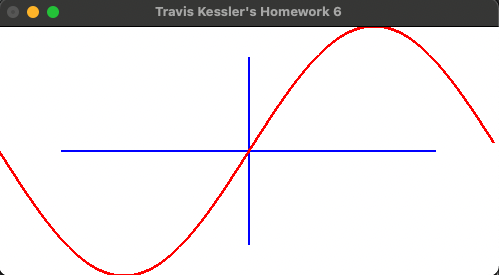
\includegraphics[scale=0.7, trim={0 0.05cm 0 0.0cm}, clip]{figures/2d_base.png}
		\caption{Default positioning for two-dimensional sinusoidal waveform}
	\end{figure}

	\begin{figure}[!ht]
		\centering
		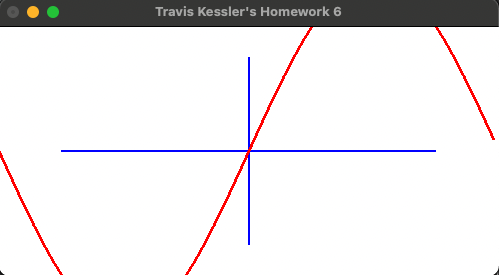
\includegraphics[scale=0.7, trim={0 0.05cm 0 0.0cm}, clip]{figures/2d_u.png}
		\caption{Increased amplitude for two-dimensional sinusoidal waveform}
	\end{figure}

	\begin{figure}[!ht]
		\centering
		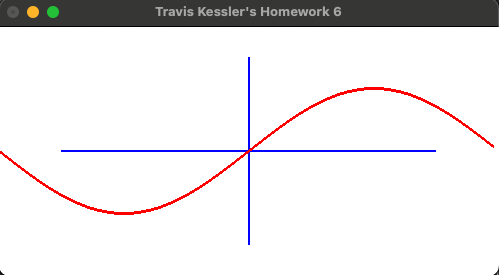
\includegraphics[scale=0.7, trim={0 0.05cm 0 0.0cm}, clip]{figures/2d_d.png}
		\caption{Decreased amplitude for two-dimensional sinusoidal waveform}
	\end{figure}

	\begin{figure}[!ht]
		\centering
		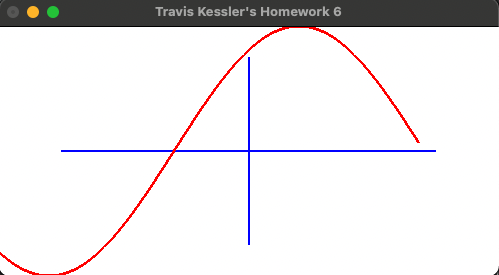
\includegraphics[scale=0.7, trim={0 0.05cm 0 0.0cm}, clip]{figures/2d_l.png}
		\caption{Left-shifted positioning for two-dimensional sinusoidal waveform}
	\end{figure}

	\begin{figure}[!ht]
		\centering
		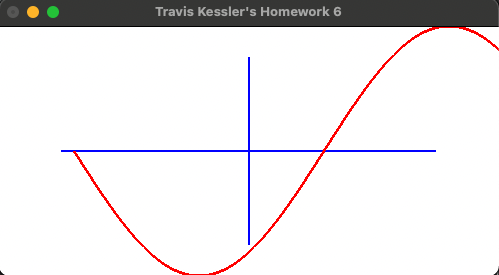
\includegraphics[scale=0.7, trim={0 0.05cm 0 0.0cm}, clip]{figures/2d_r.png}
		\caption{Right-shifted positioning for two-dimensional sinusoidal waveform}
	\end{figure}

	\begin{figure}[!ht]
		\centering
		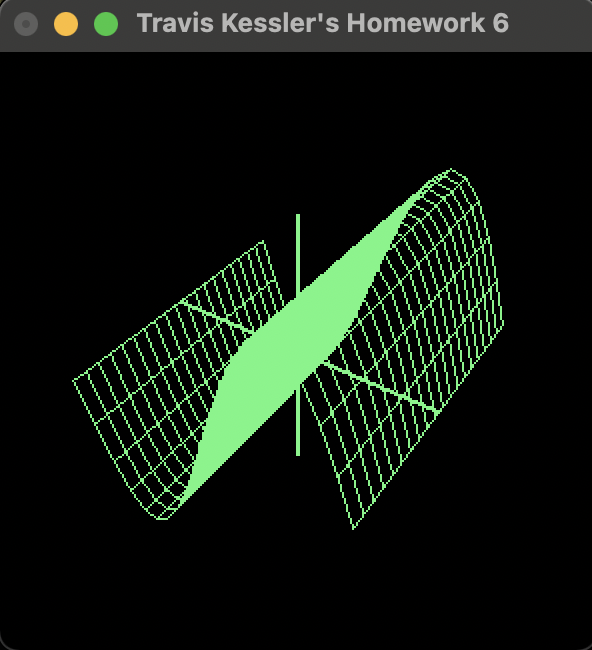
\includegraphics[scale=0.7, trim={0 0.05cm 0 0.0cm}, clip]{figures/3d_base.png}
		\caption{Default positioning for three-dimensional sinusoidal waveform}
	\end{figure}
	
	\begin{figure}[!ht]
		\centering
		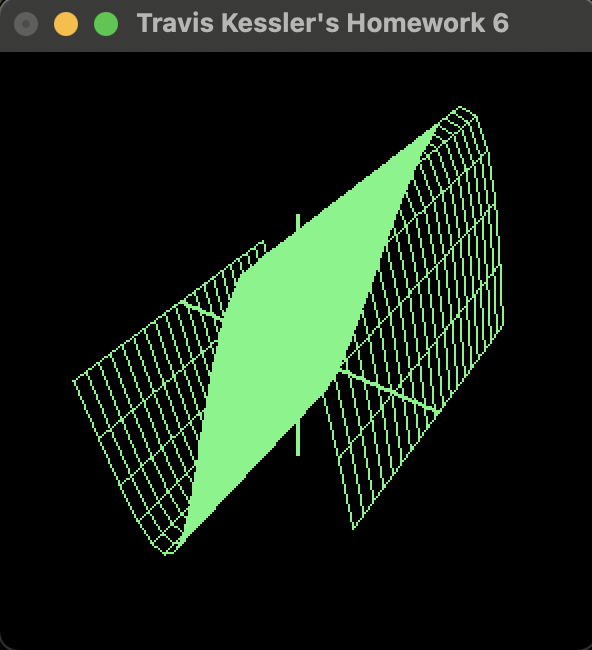
\includegraphics[scale=0.7, trim={0 0.05cm 0 0.0cm}, clip]{figures/3d_u.png}
		\caption{Increased amplitude for three-dimensional sinusoidal waveform}
	\end{figure}
	
	\begin{figure}[!ht]
		\centering
		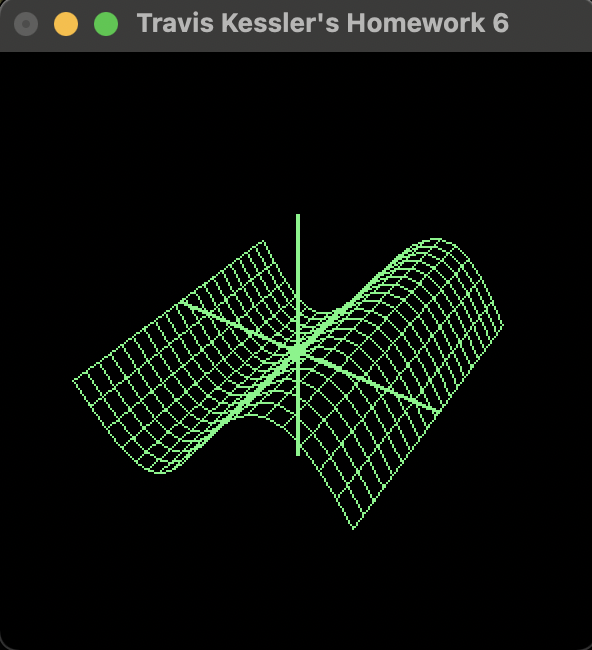
\includegraphics[scale=0.7, trim={0 0.05cm 0 0.0cm}, clip]{figures/3d_d.png}
		\caption{Decreased amplitude for three-dimensional sinusoidal waveform}
	\end{figure}
	
	\begin{figure}[!ht]
		\centering
		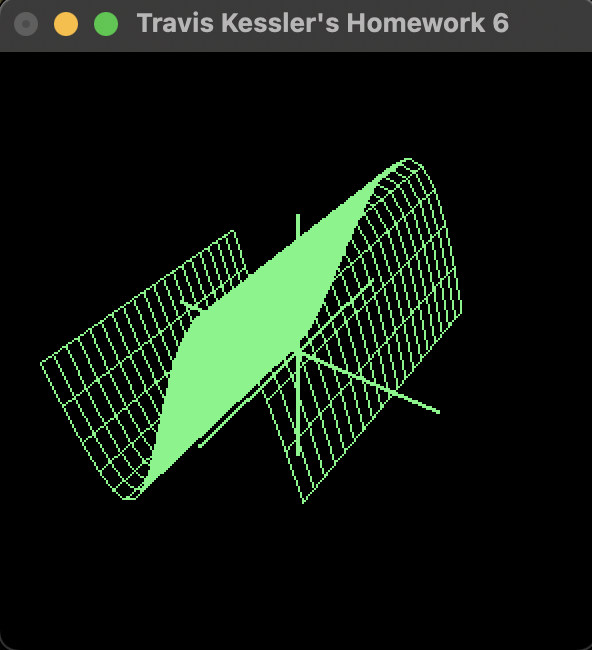
\includegraphics[scale=0.7, trim={0 0.05cm 0 0.0cm}, clip]{figures/3d_l.png}
		\caption{Left-shifted positioning for three-dimensional sinusoidal waveform}
	\end{figure}
	
	\begin{figure}[!ht]
		\centering
		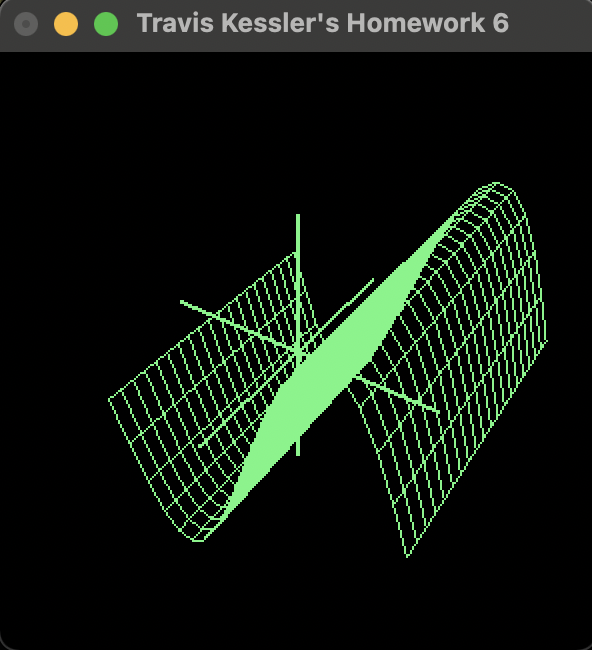
\includegraphics[scale=0.7, trim={0 0.05cm 0 0.0cm}, clip]{figures/3d_r.png}
		\caption{Right-shifted positioning for three-dimensional sinusoidal waveform}
	\end{figure}

\newpage

	\begin{thebibliography}{99\kern\bibindent}
	
	\bibitem{hwref}
	Thompson, C.
	\textit{University of Massachusetts Lowell Department of Electrical and Computer Engineering 16.520 Computer Aided Engineering Analysis Problem Set 6}.
	Retrieved April 19, 2021, from http://morse.uml.edu/Activities.d/16.520/S2021.d/ps6.pdf
	
	\end{thebibliography}

\end{document}